\chapter{Transmissão em série de dados HDMI} \label{chap:chap5}

%imp -> https://www.xilinx.com/support/answers/64340.html
Neste capítulo são contempladas todas as arquiteturas desenvolvidas para a transmissão dos dados HDMI em série, explicando todas as decisões tomadas para se obter o produto final. 

\section{Abordagem inicial}

Numa fase inicial do projeto optou-se por abordar de uma maneira simples a transmissão dos dados em série, sem o recurso à definição de todas a tramas de uma pacote. Tal decisão foi tomada, ciente da importância das tramas num protocolo de comunicação, pois o módulo GTX disponibilizado pela \textit{Xilinx} é muito complexo e completo e foi necessário uma familiarização com o mesmo.

\subsection{Transmissão de uma barra de cores gerada na FPGA em série} \label{sub:planD}

A arquitetura desenvolvida passa por um conjunto de fases que vão desde a criação do módulo GTX através da interface disponibilizada no \textit{software} para tal, e todas as tomadas de decisões que isso envolve, até a concepção de arquiteturas que criem e verifiquem as tramas. Todas essas fases serão devidamente explicadas nesta subsecção.

\subsubsection*{Considerações sobre a arquitetura} \label{subsub:planD_considerações}

A arquitetura desenvolvida gera uma barra de cores em \textit{FULL HD} na FPGA, tal como descrito em \ref{subsub:planA} no capítulo \ref{chap:chap3}, a uma taxa de atualização vertical de 60 Hz. A placa HDMI transmissora utilizada nesta arquitetura deve receber imagens no formato RGB de 30 bits e por isso está programada para a configuração por omissão, referida em \ref{subsubsec:HDMIconfigdefault} na página \pageref{subsubsec:HDMIconfigdefault}. Para além disto, a arquitetura também tem um bloco que gera as tramas e envia-as para o GTX, do mesmo modo que tem um bloco que recebe as tramas e retira a informação das mesmas, enviando-as para uma arquitetura que envie esses mesmos dados para a placa HDMI transmissora. Este diagrama geral da arquitetura esta representado na figura \ref{fig:planD_SIMPLES}.

\begin{figure}[h!]
	\begin{center}
		\leavevmode
		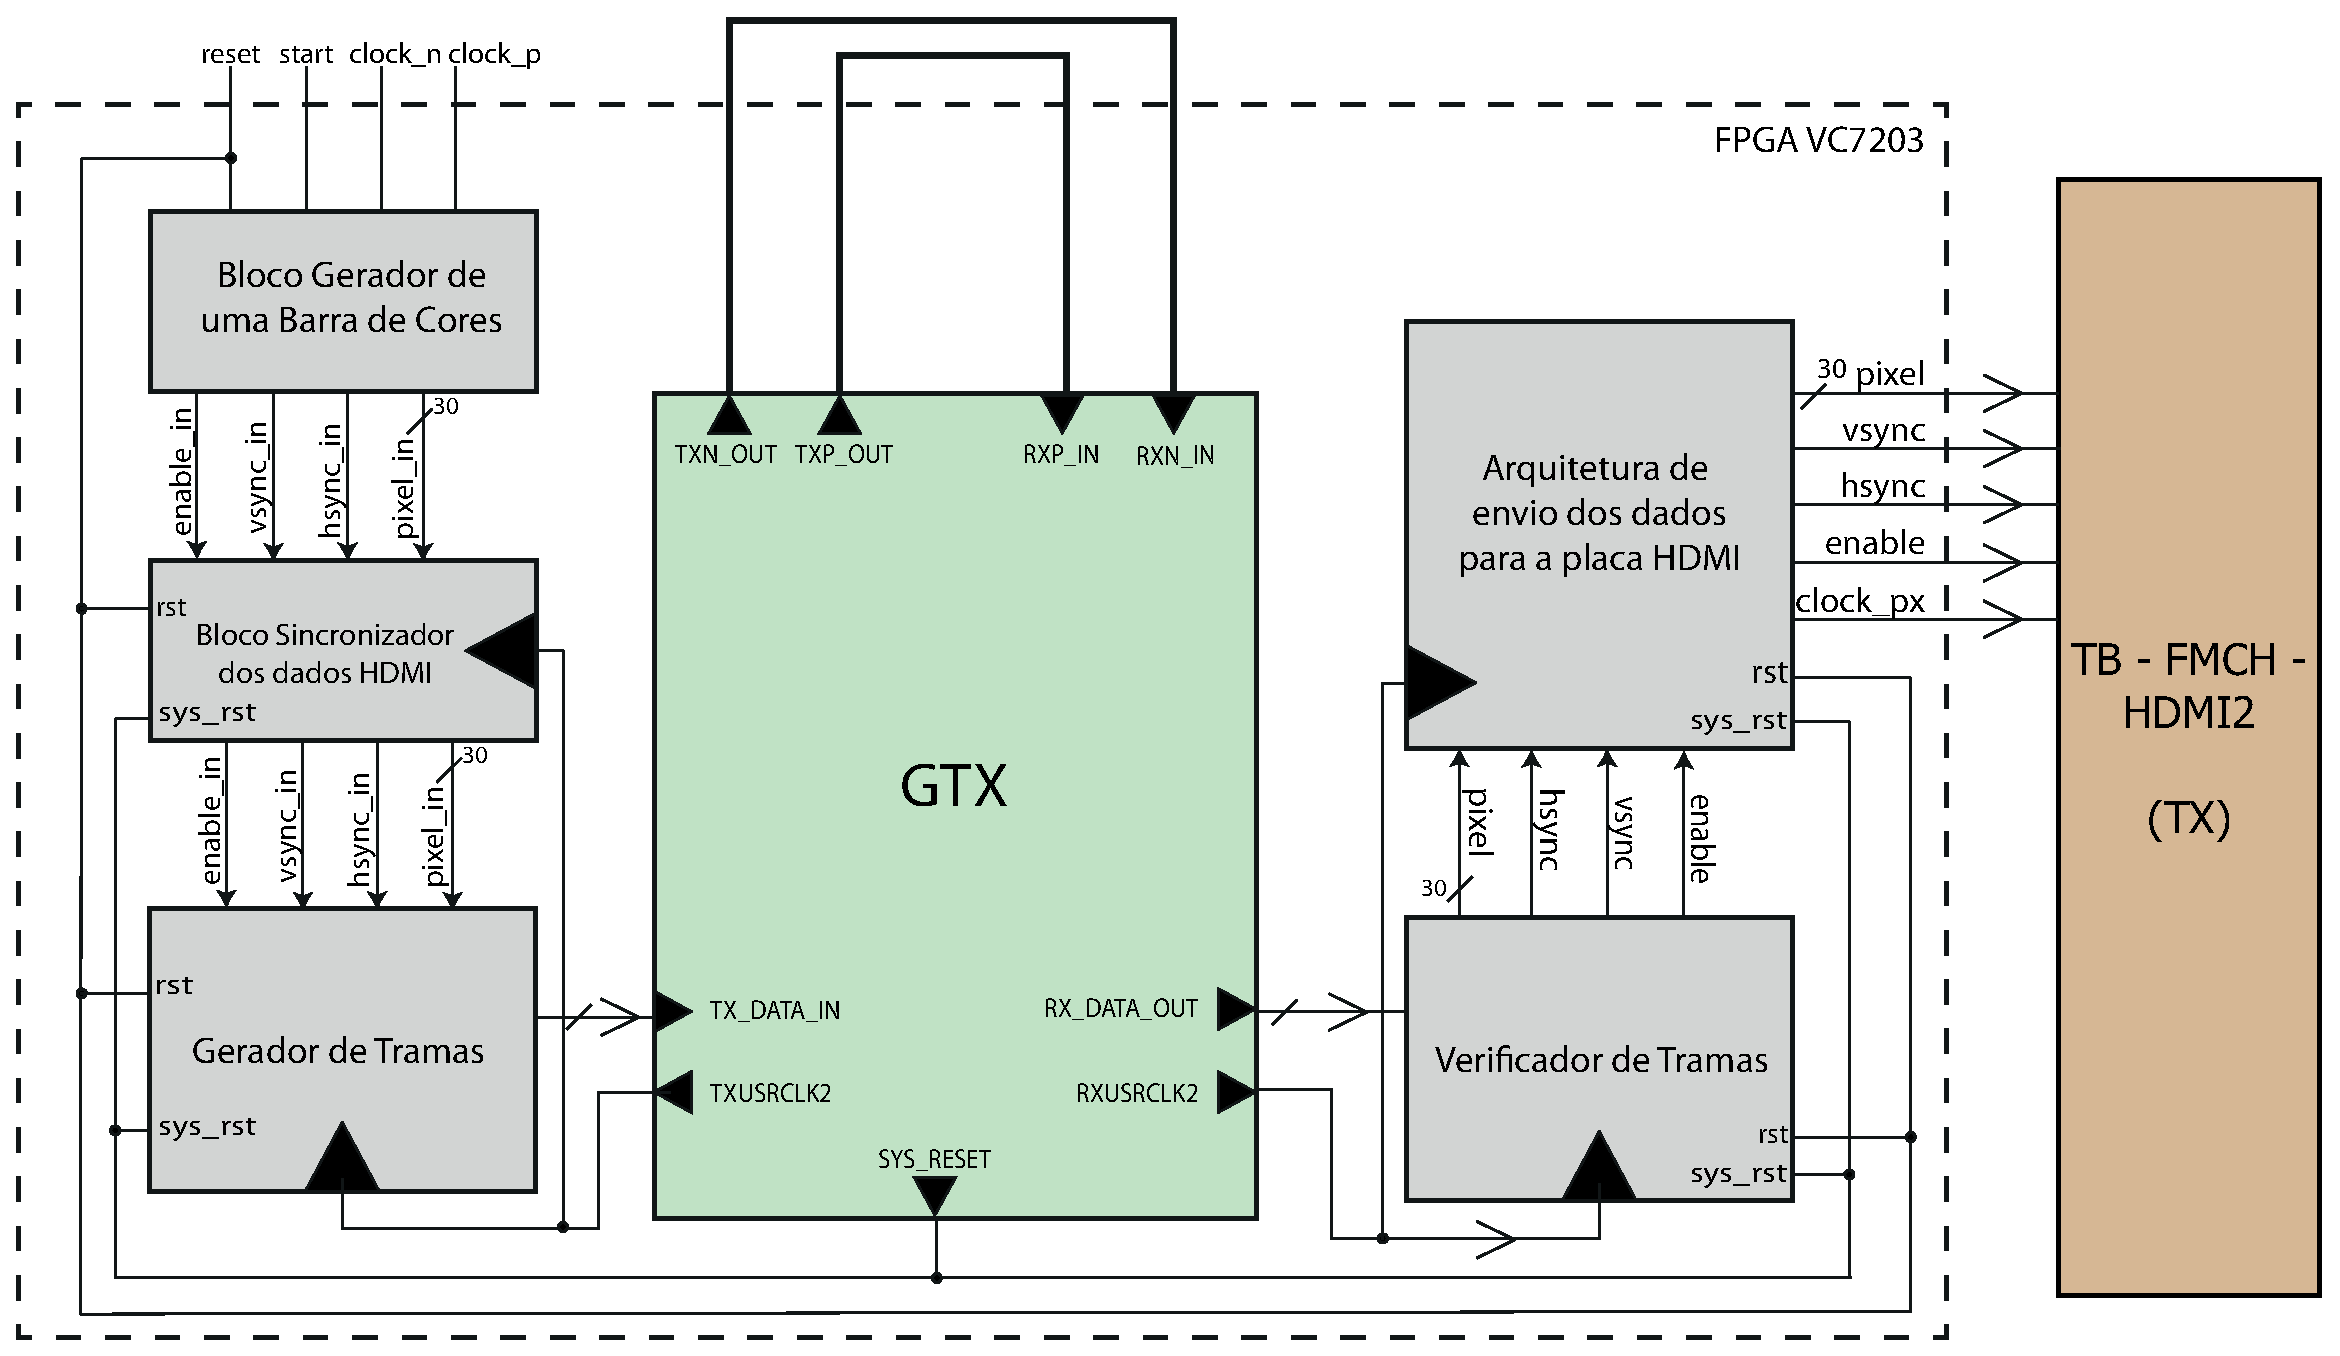
\includegraphics[width=1.0\textwidth]{planod_simples}
		\captionsetup{width=1.0\linewidth}
		\caption[Diagrama de blocos geral da arquitetura que transmite uma barra de cores em série]{Diagrama de blocos geral da arquitetura que transmite uma barra de cores em série}
		\label{fig:planD_SIMPLES}
	\end{center}
\end{figure}

Tal como é de esperar, e foi referido em \ref{sec:sincronizacao} na página \pageref{sec:sincronizacao}, os sinais de relógio provenientes do GTX e do módulo que gera a barra de cores não são o mesmo, e por isso, existe um bloco entre a geração e a criação de tramas que permite a sincronização entre os diferentes domínios de sinais de relógio através de \textit{shift-registers}.

Tendo em conta a arquitetura global desenvolvida, foram tomadas 2 decisões importantes para definir as características do transcetor: o número de bits por trama e a frequência a que estas serão lidas para o mesmo. Tal como já foi referido, a maneira mais eficiente no que toca à escolha da frequência de amostragem para o transcetor, é escolher a própria frequência da imagem HDMI, ou seja, 148,5 MHz para uma imagem \textit{FULL HD}. Relativamente ao número de bits por trama, tendo em conta que é necessário enviar os sinais todos (\textit{pixel}, \textit{vsync}, \textit{hsync} e \textit{enable}) e visto que nesta fase do projeto não houve a preocupação da criação de diferentes tramas para os diversos momentos de transmissão, escolheu-se enviar tramas de 40 bits.

Observando novamente a tabela \ref{table:line_rates} na página \pageref{table:line_rates}, independentemente do tamanho do \textit{datapath} escolhido, obtém-se uma taxa de transmissão de dados de 5,94 Gb/s.

\subsubsection*{Geração do Módulo GTX} \label{subsub:GTX_generate}

Quando se gera o módulo GTX através da interface disponibiliza pelo \textit{software} VIVADO existem algumas decisões que necessitam de ser tomadas para além das que já foram. Essas passam de seguida a ser detalhadas:

Do lado do transmissor tomaram-se as seguintes principais decisões:
\begin{enumerate}
%	\item \textbf{\textit{Line Rate:}} Como referido anteriormente é 5,94 Gb/s.
%	\item \textbf{Frequência de Amostragem das Tramas:} Assim como referido anteriormente é 148,5 MHz.
%	\item \textbf{Tamanho da interface com a FPGA:} Tal como explicado em \ref{subsub:planD_considerações} na página \pageref{subsub:planD_considerações} é 40 bits
	\item \textbf{Tamanho interno dos dados:} Esta escolha envolve o número de \textit{datapath} que são utilizados e ainda o valor da frequência de TXUSRCLK. Foi selecionado 40 bits o que implica o uso de apenas um \textit{datapath} e obtém-se as frequências de TXUSRCLK E TXUSRCLK2 idênticas.
	\item \textbf{Tipo de codificação:} Neste caso não se escolheu codificação porque não é possível (a interface com a FPGA é de 40 bits) e também numa fase inicial optou-se por simplificar o projeto.
	\item \textbf{Escolha ente \textit{Buffer} ou Bloco de Alinhamento de Fase:} Tal como indicado na secção \ref{subsub:tx_buffer} foi escolhido a utilização do \textit{buffer} uma vez que é de mais fácil utilização não requerendo o uso de lógica extra (comparativamente ao bloco de alinhamento de fase) e ainda assim é robusto.
\end{enumerate}

Do lado do recetor as principais decisões tomadas foram as seguintes:
\begin{enumerate}
	\item \textbf{Tipo de equalização:} Na subsecção \ref{subsub:rx_equalização} são apresentadas as vantagens de cada um dos tipos de equalizadores disponíveis. Apesar de este ser um projeto simples em que não se pretende inserir o sinal em canais ruidosos, optou-se por utilizar um equalizador DFE uma vez que traz mais vantagens do a utilização do equalizador LPM.
	\item \textbf{Alinhamento de palavras:} Como palavra de alinhamento escolheu-se o caractere K28.3 da tabela \ref{table:caracteres_especiais_8b10b} na página \pageref{table:caracteres_especiais_8b10b}. Contudo é necessário ter em conta que não se está a utilizar codificação e, como tal, para efetuar o alinhamento da palavra o recetor não alinhará pelo caractere K28.3 codificado, mas sim, não codificado. Ou seja, na realidade quando encontrar a palavra "7C" assume que é a palavra de alinhamento e alinha a trama para esse limite. Para além disso, optou-se por ativar a porta "RXSLIDE" que ativa o alinhamento manual dos bits, pois tal como referido em \ref{subsub:align} é de esperar que seja necessário ativar o alinhamento manual para ligações cuja taxa de débito seja superior a 5 Gb/s.
	\item \textbf{Tipo de descodificação:} Não foi utilizada nenhuma descodificação, pois do lado do transmissor também não há codificação.
	\item \textbf{Escolha ente \textit{Buffer} ou Bloco de Alinhamento de Fase:} Optou-se pela escolha do \textit{buffer}, porque no caso do recetor para além não requerer lógica extra e ter uma inicialização mais rápida (comparativamente ao bloco de alinhamento de fase), também não exige que a correcção do sinal de relógio seja realizada fora do transcetor, tal como mencionado em \ref{subsub:rx_buffer}.
\end{enumerate}

Na tabela \ref {table:sumario_planoD} é apresentada uma tabela sumário do módulo gerado. Esta tabela foi adaptada da interface que gera o módulo.

\begin{table}[h!]
	\centering
	\begin{tabular}{@{}ll@{}}
		\toprule
		\multicolumn{1}{c}{\textbf{Característica}} & \multicolumn{1}{c}{\textbf{GT}} \\ \midrule
		\textbf{TX Line Rate (Gb/s)}                & 5,94                            \\
		\textbf{TX Reference Clock (MHz)}           & 148,5                           \\
		\textbf{Enconding}                          & None                            \\
		\textbf{TX Internal Data Width}             & 40                              \\
		\textbf{TX External Data Width}             & 40                              \\
		\textbf{TXUSRCLK (MHz)}                     & 148,5                           \\
		\textbf{TXUSRCLK2 (MHz)}                    & 148,5                           \\
		\textbf{TX Buffer Enabled}                  & TRUE                            \\
		\textbf{RX Line Rate (Gb/s)}                & 5,94                            \\
		\textbf{RX Reference Clock (MHz)}           & 148,5                           \\
		\textbf{Decoding}                           & None                            \\
		\textbf{RX Internal Data Width}             & 40                              \\
		\textbf{RX External Data Width}             & 40                              \\
		\textbf{RXUSRCLK (MHz)}                     & 148,5                           \\
		\textbf{RXUSRCLK2 (MHz)}                    & 148,5                           \\
		\textbf{RX Buffer Enabled}                  & TRUE                            \\ \bottomrule
	\end{tabular}
	\caption[Sumário do módulo GTX gerado para a transmissão de uma barra de cores gerada na FPGA]{Sumário do módulo GTX gerado para a transmissão de uma barra de cores gerada na FPGA (adaptada do \textit{software})}
	\label{table:sumario_planoD}
\end{table}

\subsubsection{Concepção e Desenvolvimento}

Na imagem \ref{fig:planD_SIMPLES} da página \pageref{fig:planD_SIMPLES} é representado um protótipo da arquitetura geral apresentada. Nesta subsecção são apresentados com detalhe todos os blocos utilizados e suas entradas e saídas para que se possa perceber as ligações entre os mesmos. 

\subsubsection*{Bloco gerador de uma Barra de Cores} \label{subsub:serial_colorBarGenerator}

Este bloco gerador de barra de cores é exatamente igual ao bloco descrito em \ref{subsub:planA} na página \pageref{subsub:planA}: gera uma barra de cores em \textit{FULL HD} com uma frequência de 148,5 MHz. Nas suas entradas encontram-se as portas vindas diretamente do exterior, tal como nas outras arquiteturas que utilizam este bloco, que são botões definidos pelo utilizador (\textit{reset} e \textit{start}) e também um sinal de relógio diferencial de 200 MHz. Este bloco coloca nas suas saídas sinais que são enviados para um bloco sincronizador dos dados HDMI que é de seguida detalhado.

\subsubsection*{Bloco Sincronizador dos dados HDMI} \label{subsub:serial_syncsignals}

O recurso a este bloco sincronizador dos dados HDMI é necessário devido aos diferentes domínios de relógio que existem no sistema: por um lado existe um bloco que gera uma barra de cores a uma determinada cadência, e por outro existe um bloco que gera as tramas a serem enviadas para o transcetor a outra cadência. Estes dois sinais de relógio podem ser iguais, no entanto podem não estar em fase o que é suficiente para haver problemas de meta-estabilidade. 

Por este motivo, este bloco de sincronização é apenas constituído por dois registos de deslocamento (\textit{shift-registers}) para que problemas de sincronização que possam eventualmente existir sejam resolvidos, tal como apresentado na figura \ref{fig:sync_block}. 
\begin{figure}[h!]
	\begin{center}
		\leavevmode
		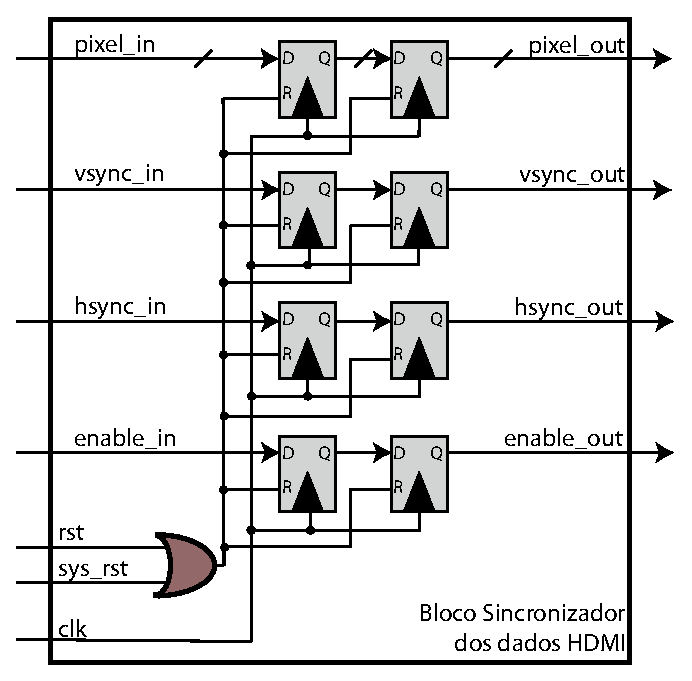
\includegraphics[width=0.6\textwidth]{sync_block}
		\captionsetup{width=1.0\linewidth}
		\caption[Bloco de sincronização de dados]{Bloco de sincronização de dados}
		\label{fig:sync_block}
	\end{center}
\end{figure}

Tal como se visualiza na figura, para além de nas suas entradas se encontrar os dados provenientes da fonte HDMI (que nesta arquitetura é o bloco gerador de barra de cores), há também dois sinais : \textit{rst} e \textit{sys\_rst}. O primeiro sinal refere-se ao sinal de \textit{reset} controlado pelo utilizador e o segundo corresponde a um sinal de \textit{reset} ativado automaticamente pelo módulo GTX.

O sinal de relógio a que opera este bloco trata-se do sinal de relógio proveniente do módulo GTX, tal como se visualiza na figura \ref{fig:planD_SIMPLES} na página \pageref{fig:planD_SIMPLES}.

\subsubsection*{Gerador de Tramas} \label{subsub:serial_frameGenerator}

Este bloco é responsável pela criação das tramas de 40 bits a serem enviadas para o módulo GTX. Relembra-se que nesta abordagem inicial do projeto não se teve em conta a criação de tramas bem definidas para todos os momentos de transição, apenas se definiu a trama que corresponde ao início de transmissão para que fosse possível do lado do recetor manter o alinhamento das tramas. 

%%Explicar trama de SOP, qdo é enviada e pq tem aquele padrão
A trama que define o início da transmissão (SOP - \textit{Start of Packet}) é uma trama que serve essencialmente para o alinhamento das palavras do lado do recetor. Ou seja, são aproveitados momentos de transmissão nulos para enviar esta trama e alinhar a mesma. Isto porque neste momento se está a lidar com uma taxa de transmissão superior a 5 Gb/s e por isso é de esperar que é necessário do lado do recetor verificar se as tramas estão realmente alinhadas.
Esta trama SOP são 40 bits que em hexadecimal corresponde a: $000605047c$. Para além de ter sido a trama de SOP sugerida pelo exemplo que a \textit{Xilinx} disponibiliza, esta trama tem as seguintes particularidades:
\begin{enumerate}
	\item No final da mesma se encontra a palavra de alinhamento(são os primeiros bits a ser transmitidos), que permite ao transcetor alinhar a trama internamente.
	\item A trama numa vista geral nunca será encontrada no meio de outros dados, que será de seguida explicado
\end{enumerate}

Esta trama é transmitida sempre que os sinais de controlo se encontram inativos, ou seja que as seguintes condições se verificarem:
\begin{enumerate}
	\item $vsync = 0$
	\item $hsync = 0$
	\item $enable = 0$
\end{enumerate}


%%Explicar como são os pacotes noutras alturas de transmissão sem ser qdo se envia SOP
Quando estas três condições não se verificam em conjunto, então é porque há algum sinal de imagem ativo, e por isso é transmitida uma trama com o formato que se visualiza na figura \ref{fig:trama_abordagem_inicial}.

\begin{figure}[h!]
	\begin{center}
		\leavevmode
		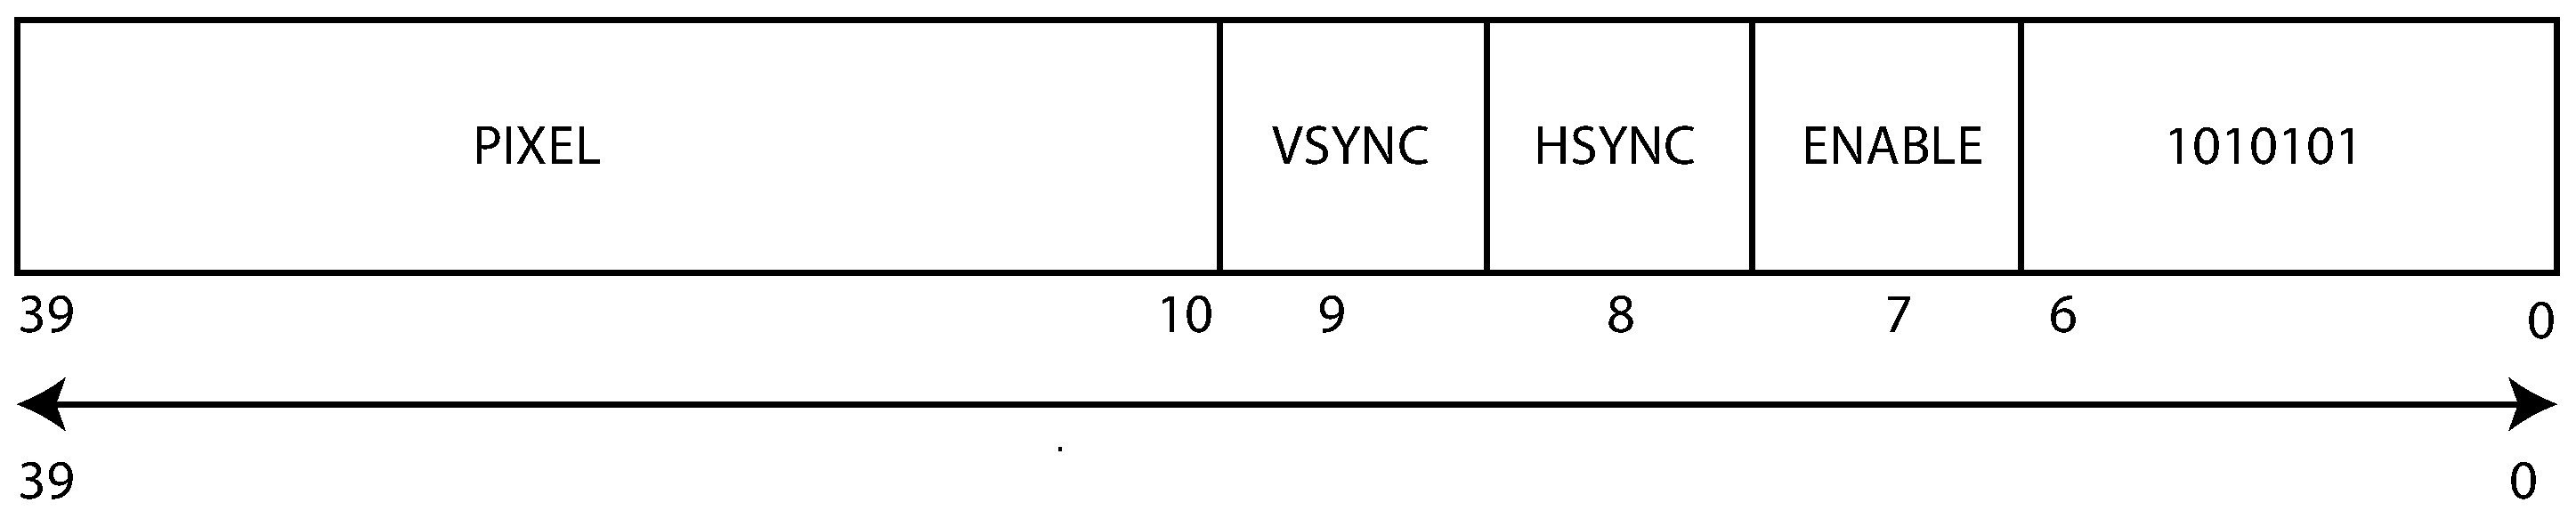
\includegraphics[width=0.9\textwidth]{trama_abordagem_inicial}
		\captionsetup{width=1.0\linewidth}
		\caption[Estrutura das tramas geradas]{Estrutura das tramas geradas}
		\label{fig:trama_abordagem_inicial}
	\end{center}
\end{figure}

Este formato de trama vem validar aquilo que foi dito anteriormente quando se justificou o formato da trama SOP: os últimos 7 bits da trama SOP são $1111100$, enquanto que os últimos 7 bits de todas as outras tramas são $1010101$. Portanto, em conjunto com o bloco verificador de tramas que garante que as tramas estão sempre alinhadas, dificilmente a trama SOP será encontrada no meio dos dados transmitidos enquanto dados da transmissão e não como trama de alinhamento.


Assim sendo, consoante os dados que recebe nas suas entradas (\textit{pixel}, \textit{vsync}, \textit{hsync} e \textit{enable}), este bloco ou envia SOP ou envia tramas no formato da imagem \ref{fig:trama_abordagem_inicial}. A imagem \ref{fig:momentos_tramas} exemplifica os diversos momentos de transmissão das diferentes tramas numa imagem. A cinza correspondem os momentos da imagem em que os sinais de controlo estão inativos, e por isso são transmitidos SOP, e a castanho correspondem os momentos de transmissão em que algum dos sinais de controlo está ativo e por isso são enviadas tramas no formato previamente exemplificado. Sempre o sinal \textit{rst} ou \textit{sys\_rst} estiver ativo então os dados são repostos e as tramas enviadas são SOP. 

\begin{figure}[h!]
	\begin{center}
		\leavevmode
		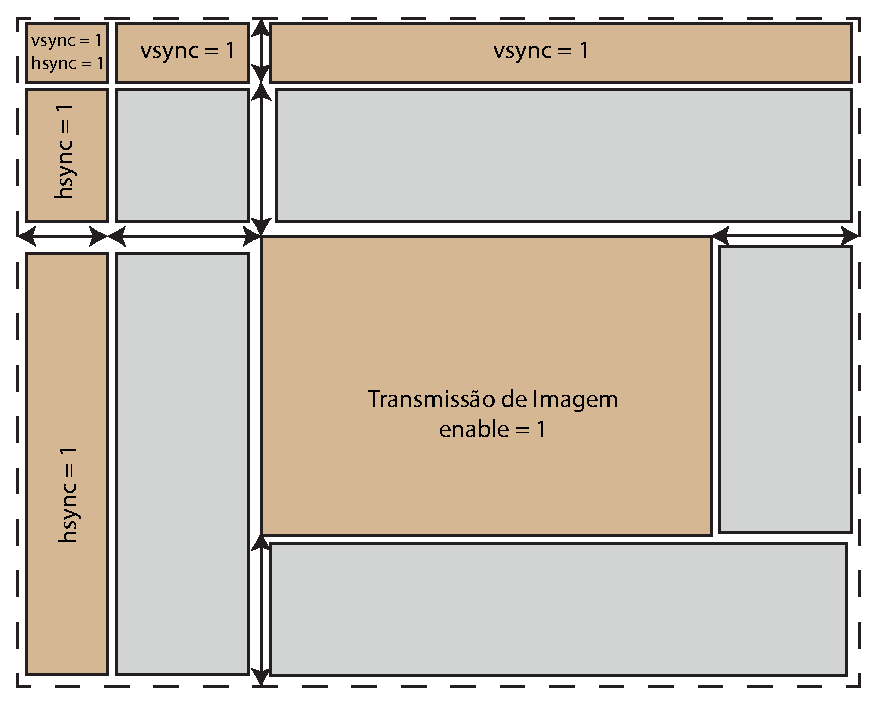
\includegraphics[width=0.7\textwidth]{exemplo_tramas_transmissoes}
		\captionsetup{width=1.0\linewidth}
		\caption[Momentos de transmissão de diferentes tramas]{Momentos de transmissão de diferentes tramas}
		\label{fig:momentos_tramas}
	\end{center}
\end{figure}

É de esperar que a transmissão demore algum tempo a alinhar do lado do recetor, e por isso, é necessário que as tramas SOP sejam enviadas durante algum tempo, por isso se escolheram os momentos de transição de dados de controlo nulos, pois são suficientemente longos para que as tramas possam ser alinhadas. Assim, no pior dos casos, perde-se a primeira imagem completa que é transmitida, pois não são recebidos os primeiros dados de controlo (\textit{vsync} e \textit{hsync}) mas garanta-se que todas as outras estão alinhadas e os dados serão corretamente recebidos do lado do transmissor.

\subsubsection*{Verificador de Tramas} \label{subsub:serial_frameChecker}
  
%%Explicar porque existe

Este bloco é responsável pela re-organização das tramas recebidas que são recebidas à cadência RXUSRCLK2. Apesar de poder parecer que com o alinhamento interno as tramas chegariam ao recetor tal como são enviadas do transmissor, mesmo com o alinhamento interno ideal, tal não acontece. As tramas são sim alinhadas consoante determinada palavra de alinhamento, no entanto não significa que a trama recebida é exatamente à trama enviada. 

O que o alinhamento interno faz, segundo \cite{R022} e \cite{R011}, quando deteta a palavra de alinhamento é assumir que dessa palavra para a frente são dados válidos, tal como explicado anteriormente, e alinhar os dados para um determinado limite. Esse limite pode ser selecionado aquando a criação do módulo na interface especifica para tal, e o que foi escolhido é que alinha os dados para o byte mais próximo. Apesar de não se estar a lidar com codificação, o bloco de alinhamento das palavras considera que 1 byte são 10 bits (pois com a codificação 8B/10B codifica 8 bits em 10 bits) porque o \textit{datapath} é de 40 bits, e por isso quando deteta a palavra de alinhamento, as tramas recebidas no recetor podem chegar de 4 maneiras diferentes ilustradas na imagem \ref{fig:alinhamento_tramas_gtx}.


%Se o datapath fosse de 32 bits sem codificação, assumiria que 1 byte sao 8 bits, de certeza, apesar de eu nao ter testado
\begin{figure}[h!]
		\begin{center}
		\leavevmode
		\includegraphics[width=0.8\textwidth]{organizacao_tramas}
		\captionsetup{width=1.0\linewidth}
		\caption[Alinhamento das tramas no transcetor]{Alinhamento das tramas no transcetor}
		\label{fig:alinhamento_tramas_gtx}
	\end{center}
\end{figure}

Daí a importância da trama de SOP: quando é detetada em algum dos limites assinalados a cinzento então dá-se inicio à transmissão dos restantes dados. Para se proceder à organização dos dados recebidos, é necessário recorrer a uma máquina de estados. Esta máquina de estados utilizada neste exemplo foi adaptada de uma máquina de estados disponibilizada pela \textit{Xilinx}.

A máquina de estados principal é dividida em 3 por questões de simplificação e de melhor entendimento:
\begin{enumerate}
	\item Máquina que define o estado dos dados recebidos
	\item Máquina que define o estado da procura dos dados de tramas e procede a eventuais re-alinhamentos de palavras necessários
	\item Máquina que deteta os erros 
	\item Máquina que deteta o estado da ligação
\end{enumerate}

Cada uma delas passará a ser detalhada, sem nunca esquecer que funcionam como um todo apenas foram divididas para explicação do sistema global.
%%Explicar máquina de estados que procura dados, ou espera ou tal e tal

\begin{enumerate}
	\item \textbf{Máquina que define o estado dos dados recebidos}
	\item \textbf{Máquina que define o estado da procura dos dados de tramas e procede a eventuais re-alinhamentos de palavras necessários}
	\item \textbf{Máquina que deteta os erros }
	\item \textbf{Máquina que deteta o estado da ligação}
\end{enumerate}

%%Explicar maquina de estados que ativa o RXSLIDE (que alinha caso o sinal esteja falsamente alinhado)
%Tal como já foi mencionado várias vezes ao longo do documento, para taxas de transmissão superiores a 5 Gb/s, o 
%%Explicar máquina de estados que a
  
%\subsubsection*{Bloco de envio de dados para a placa HDMI} \label{subsub:serial_send signals to HDMI}

%\subsubsection*{Localizações das portas de saída do módulo de topo} \label{subsub:serial_locs_planD}
%%%falar das portas todas
%
%%%falar das constraints físicas
%
%%%falar das constrainsts temporais
%
%\subsubsection*{Resultados} \label{subsub:serial_planDresults}
%\begin{figure}[h!]
%	\begin{center}
%		\leavevmode
%		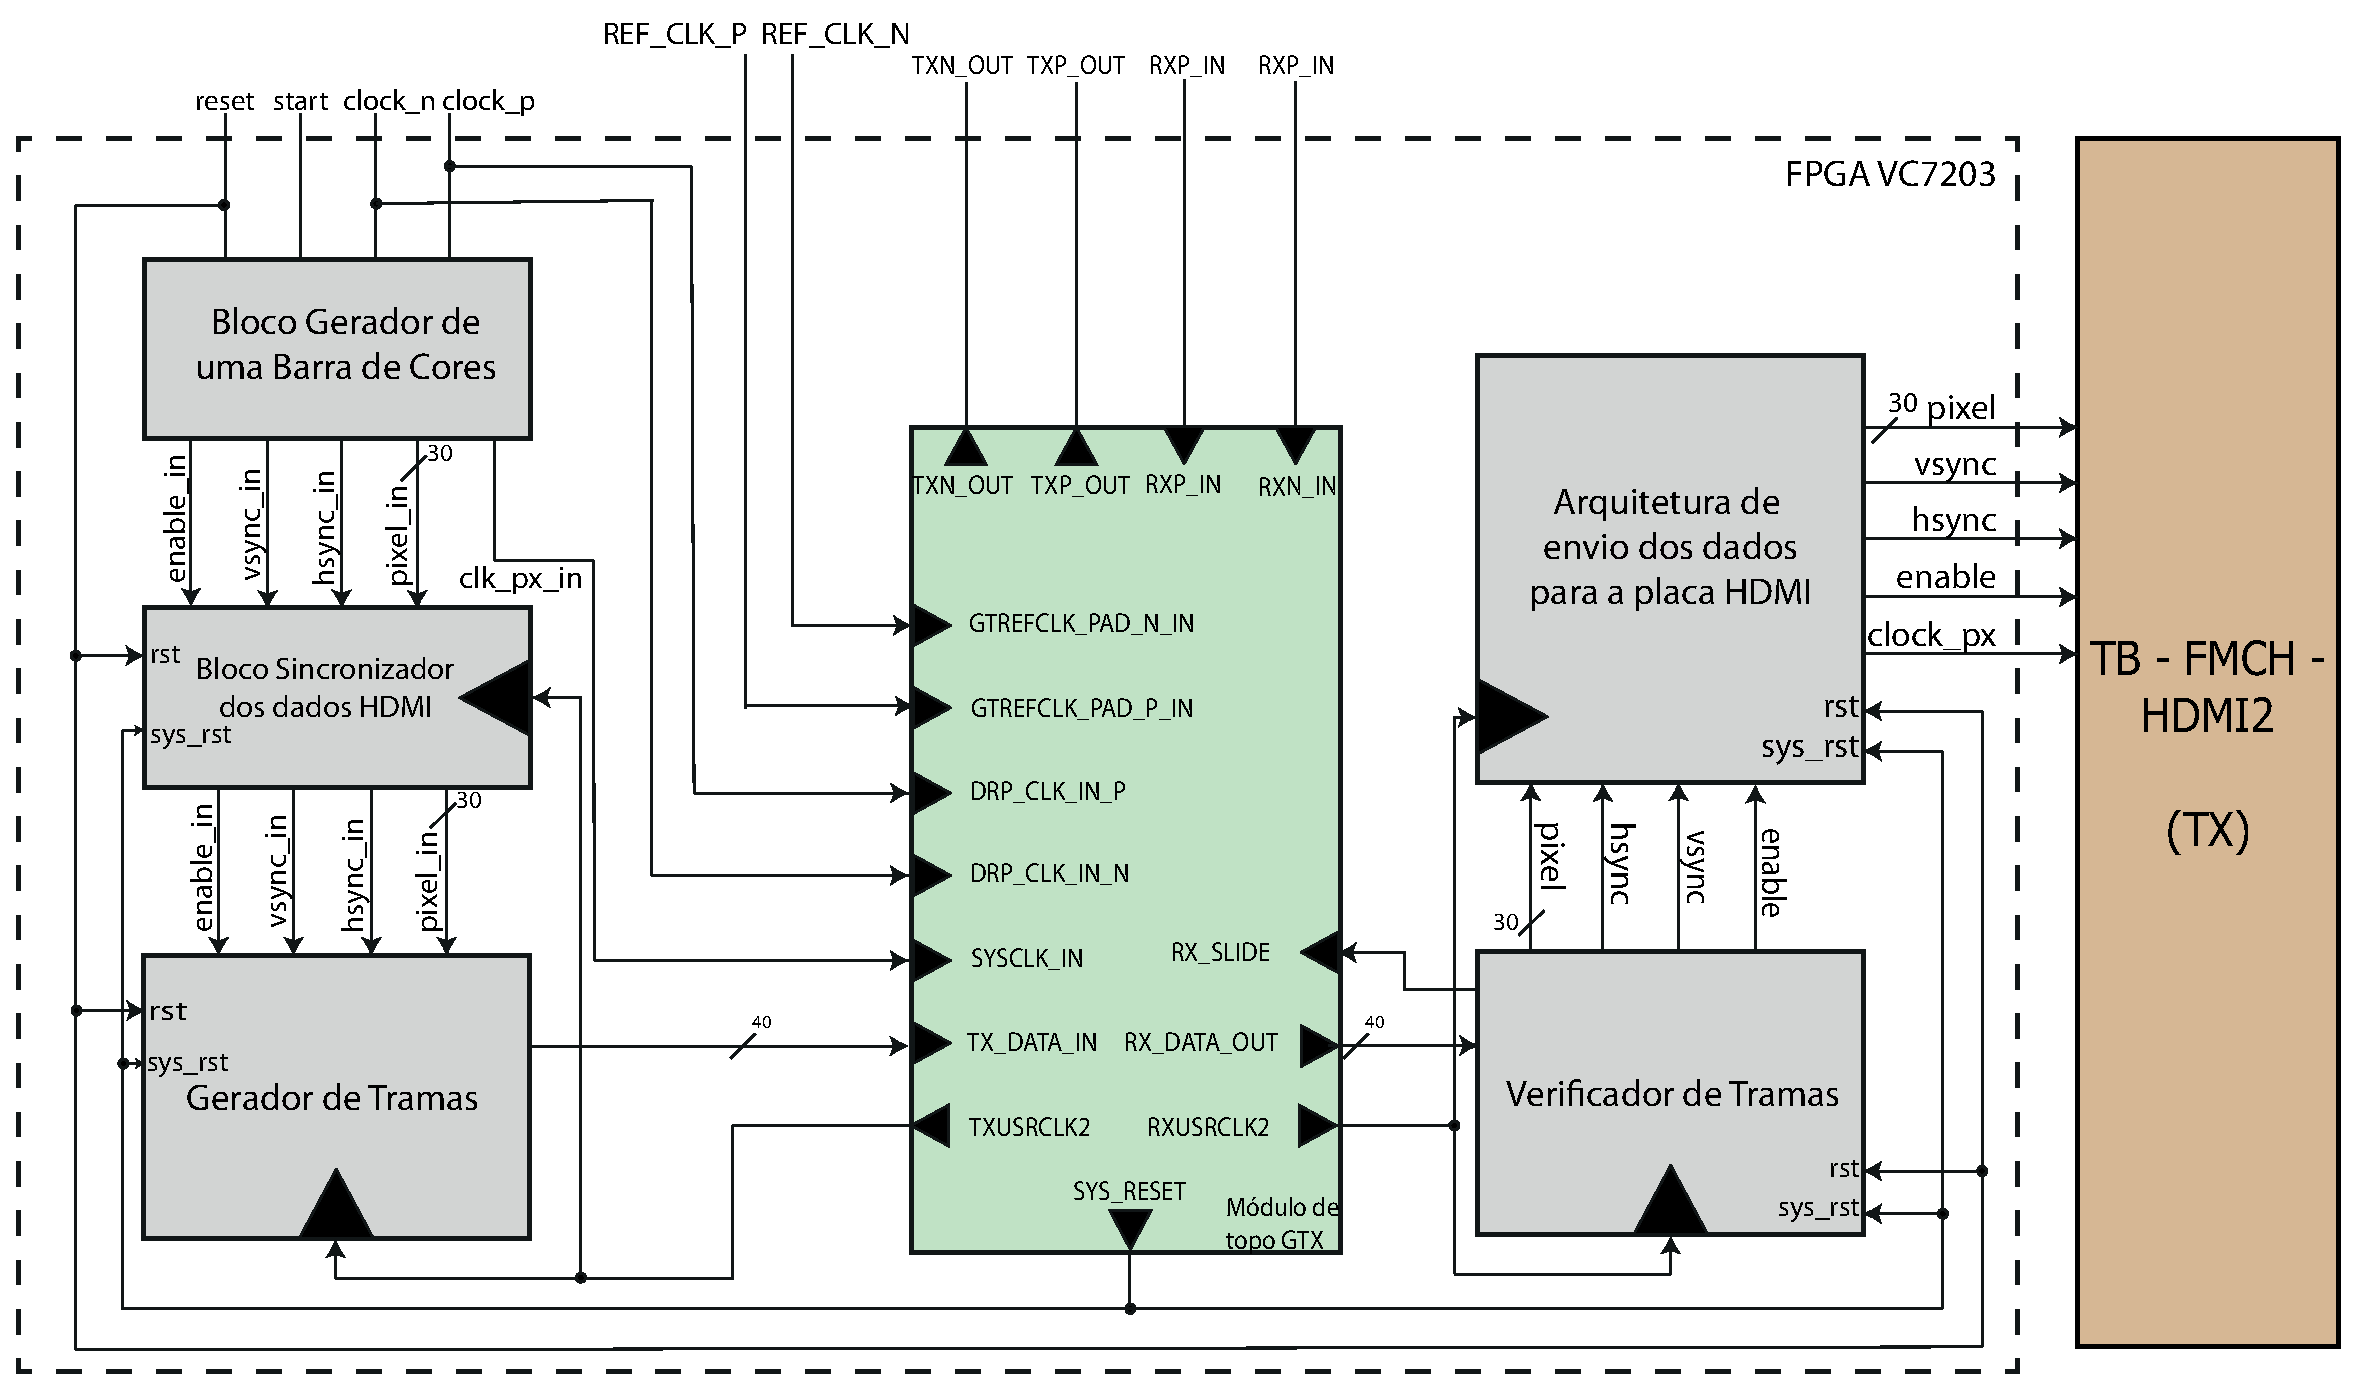
\includegraphics[width=1.0\textwidth]{planod}
%		\captionsetup{width=1.0\linewidth}
%		\caption[Diagrama de blocos da arquitetura de transmissão em série de uma barra de cores gerada na FPGA]{Diagrama de blocos da arquitetura de transmissão em série de uma barra de cores gerada na FPGA}
%		\label{fig:planD}
%	\end{center}
%\end{figure}
%
%\subsection{Transmissão de imagem em série entre dispositivos HDMI} \label{sub:planE}
%
%\subsubsection*{Considerações sobre a arquitetura} \label{subsub:planE_considerações}
%\begin{figure}[h!]
%	\begin{center}
%		\leavevmode
%		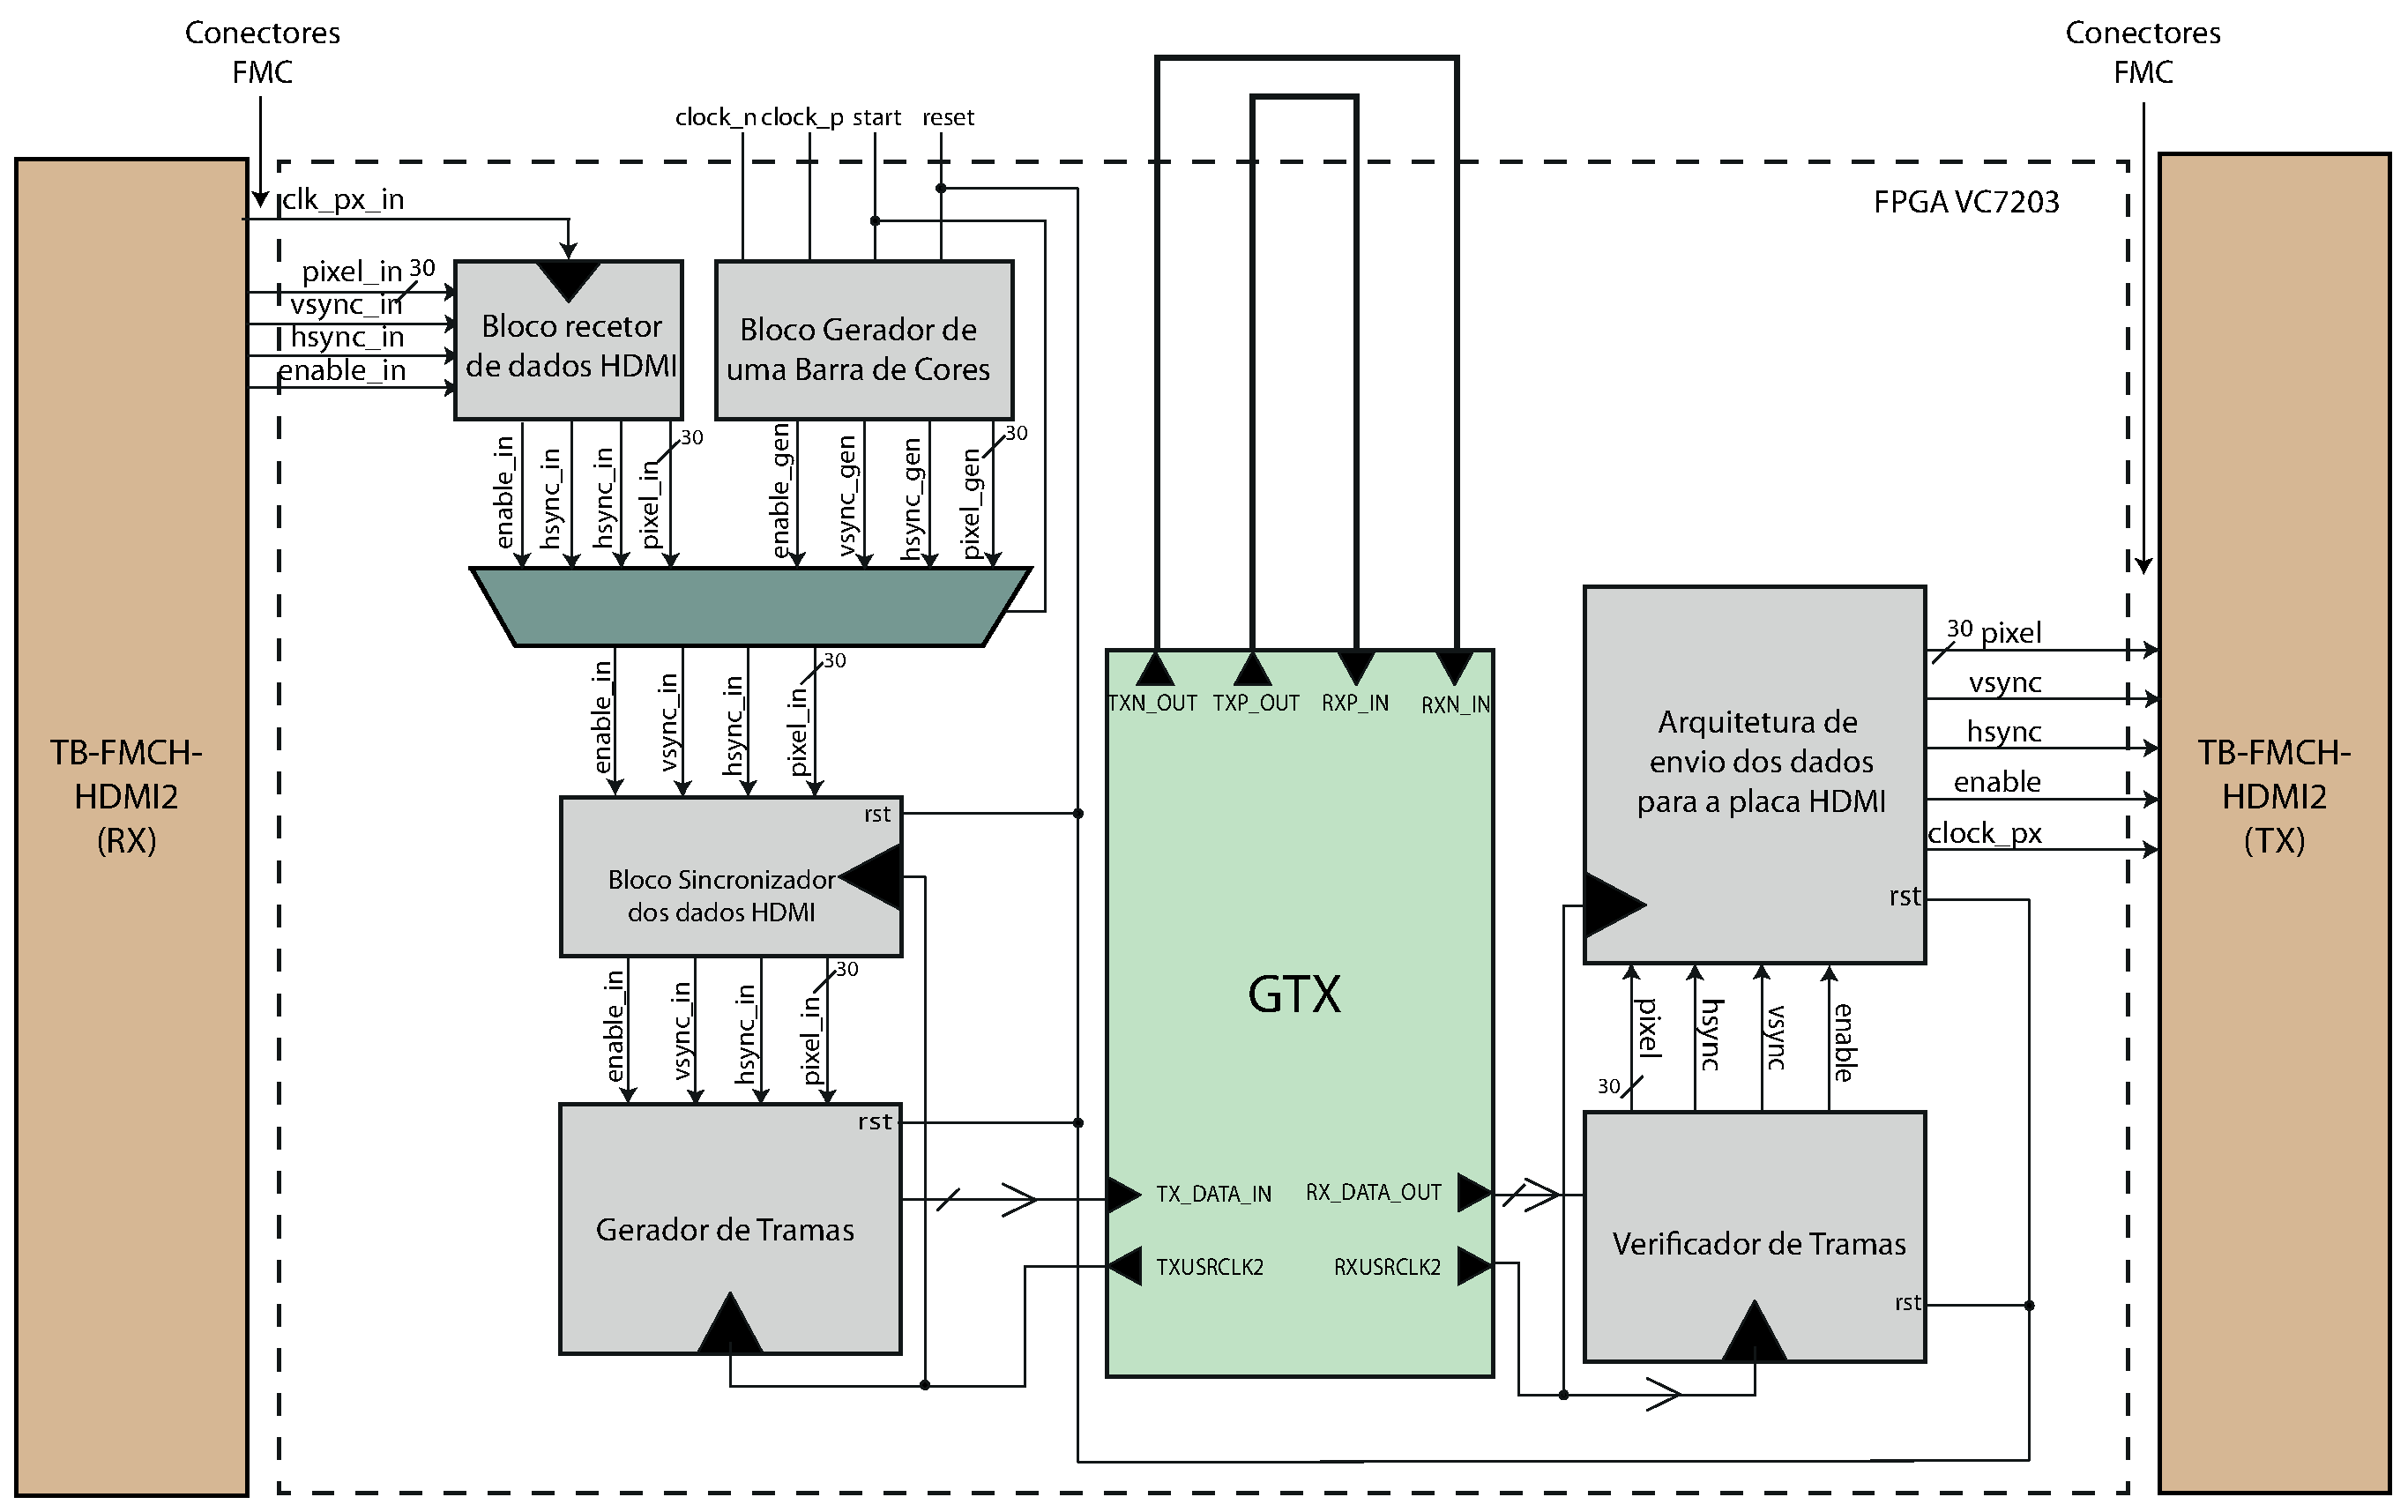
\includegraphics[width=1.0\textwidth]{planoE_simples_pt}
%		\captionsetup{width=1.0\linewidth}
%		\caption[]{}
%		\label{fig:planE_simples}
%	\end{center}
%\end{figure}
%%\section{Arquiteturas Desenvolvidas}
%%
%%\subsection{Transmissão em série de uma imagem gerada na FPGA para um dispositivo HDMI de destino}
%%
%%\subsection{Transmissão em série imagem entre dispositivos HDMI}